\documentclass[12pt]{article}

% Pacchetti necessari
\usepackage[utf8]{inputenc}
\usepackage[italian]{babel}
\usepackage{graphicx}
\usepackage{adjustbox}
\usepackage{tabularx}
\usepackage{makecell}
\usepackage{listings}
\usepackage{color}
\usepackage{hyperref}
\usepackage{geometry}
\usepackage{amsmath}
\usepackage{xcolor}
\usepackage{tikz}
\usepackage{pgfplots}
\usepackage{siunitx}
\pgfplotsset{compat=1.17}

\newcommand{\coloredbox}[1]{%
  \textcolor[HTML]{#1}{\rule{1.5ex}{1.5ex}}\hspace{0.3em}}

% Configurazione per il codice sorgente
\lstset{
  basicstyle=\ttfamily,
  columns=fullflexible,
  frame=single,
  breaklines=true,
  postbreak=\mbox{\textcolor{red}{$\hookrightarrow$}\space},
}

% Impostazioni di geometria della pagina
\geometry{
 a4paper,
 total={170mm,257mm},
 left=20mm,
 top=20mm,
}


\begin{document}

\begin{titlepage}
   \centering
   \includegraphics[width=6cm]{Uniroma1.svg.png} 
   \vspace{1cm}

   {\scshape\LARGE Università "Sapienza" di Roma \par}
   \vspace{0.5cm}
   {\scshape\Large Facoltà di Informatica\par}
   \vfill

   \rule{\textwidth}{1pt}\vspace*{-\baselineskip}\vspace*{2pt}
   \rule{\textwidth}{0.4pt}\\[\baselineskip]

   {\LARGE \bfseries Rendering con Raytracing\par}

   \rule{\textwidth}{0.4pt}\vspace*{-\baselineskip}\vspace{2pt}
   \rule{\textwidth}{1pt}\\[\baselineskip]

   \vfill

\begin{tikzpicture}[remember picture,overlay]
   \node[anchor=south west,inner sep=0pt] at ([xshift=3cm,yshift=3.7cm]current page.south west) {
      \begin{tikzpicture}
         \clip (1,1) circle (1cm); % Adjust the radius for the size of the circle
         \node[anchor=south west,inner sep=0pt] at (0,0) {\includegraphics[width=2cm]{dev duo lgoo.png}};
      \end{tikzpicture}
   };
\end{tikzpicture}

   {\Large\itshape Cirelli Samuele\par}
   {\Large\itshape Fiorelli Federico\par}

   \vspace{1.5cm}

   {\large 28 gennaio 2024\par}
\end{titlepage}

\tableofcontents
\newpage

\section{Introduzione}
Il presente documento descrive lo sviluppo e l'implementazione di un progetto avanzato in linguaggio di programmazione C++, focalizzato sulla creazione di un sistema di rendering. Questo si propone di esplorare le capacità del C++ nel gestire applicazioni grafiche complesse, con particolare attenzione verso l'elaborazione e la visualizzazione di elementi 3D.

Nel contesto dell'informatica grafica e della simulazione, il rendering è un processo cruciale che trasforma modelli 3D e altre forme di dati astratti in immagini visivamente comprensibili e realistiche. Questo progetto, pertanto, non solo serve per dimostrare le potenzialità del C++ in questo ambito, ma mira anche a fornire soluzioni innovative e ottimizzate per le sfide comuni incontrate nel rendering grafico.

Il sistema di rendering sviluppato in questo progetto si avvale di diverse librerie e tecnologie moderne: al suo cuore vi è la manipolazione di strutture geometriche, luci, ombre e materiali, il tutto gestito attraverso un'architettura software ben progettata e modulare. Questo approccio non solo garantisce la flessibilità e l'espandibilità del sistema ma permette anche un'efficace gestione delle risorse, un aspetto fondamentale per applicazioni grafiche ad alte prestazioni.

L'obiettivo di questa relazione è di documentare in modo esaustivo il processo di sviluppo del progetto, dalla fase di concezione e progettazione fino all'implementazione e ai test dei vari moduli. Verranno analizzate le scelte architetturali, le strategie di ottimizzazione adottate e le soluzioni ai problemi incontrati durante lo sviluppo. Inoltre, saranno presentati dei benchmark per dimostrare l'efficacia del sistema di rendering realizzato.

Attraverso questo progetto si intende contribuire al campo dell'informatica grafica, fornendo un esempio concreto di come il linguaggio C++, con le sue caratteristiche di potenza e flessibilità, possa essere impiegato per costruire soluzioni software avanzate e performanti in questo settore in rapida evoluzione.

\section{Sviluppo}


\subsection{Design del Renderer}
Il file \textit{renderer.h} rappresenta il cuore del nostro sistema di rendering, incorporando le funzionalità principali richieste per generare immagini 3D realistiche da strutture di dati geometriche. Il renderer è stato progettato con un approccio modulare, consentendo una facile integrazione e scalabilità con diverse architetture hardware, inclusi i sistemi multi-thread su CPU e i dispositivi basati su CUDA.

\subsubsection{Architettura Generale}
L'architettura del renderer è stata sviluppata per essere sia efficiente che flessibile. Si basa su una serie di componenti chiave che lavorano in armonia per elaborare i dati 3D e trasformarli in immagini bidimensionali.
Questi componenti includono la gestione della camera, la definizione dei materiali, la gestione della luce e delle geometrie \textit{hittable}, insieme alla matematica sottostante fornita dalla libreria \textit{GLM}.

\subsubsection{Componenti Chiave}
\begin{itemize}
\item \textbf{Camera}: La camera è fondamentale per definire la vista e la prospettiva all'interno della scena 3D. Le sue proprietò determinano come gli oggetti 3D vengono proiettati sull'immagine finale.

\item \textbf{Materiali}: I materiali definiscono le proprietà di superficie degli oggetti, come il colore, la riflessione, la rifrazione e l'emissione di luce. Questi elementi sono cruciali per il calcolo di colore e dell'intensità della luce che colpisce ogni punto della scena.

\item \textbf{Luci}: Le luci sono gestite in modo da determinare come illuminano gli oggetti nella scena, influenzando direttamente le ombre, i riflessi e l'aspetto generale dell'immagine.

\item \textbf{Geometrie Hittable}: Le geometrie hittable rappresentano gli oggetti 3D nella scena. Ogni oggetto ha la capacità di interagire con i raggi di luce, determinando come vengono visualizzati nell'immagine finale.
\end{itemize}

\subsubsection{Algoritmo di Ray Tracing}
Il nucleo dell'algoritmo di ray tracing è implementato nella funzione \textit{TraceRay}. Questa funzione calcola ricorsivamente il percorso di un raggio attraverso la scena, determinando i punti di intersezione con gli oggetti e calcolando il colore risultante in base ai materiali e alle proprietà di luce. L'algoritmo tiene conto di riflessioni, rifrazioni e ombre, permettendo la creazione di immagini realistiche.

\subsubsection{Anti-Aliasing}
Per migliorare la qualità dell'immagine finale e ridurre l'effetto di aliasing, è implementata la tecnica di anti-aliasing. Questa tecnica media i colori di più campioni per pixel, risultando in immagini più levigate e realistiche.

\subsubsection{Ottimizzazioni e Scalabilità}
Il renderer è progettato con l'obiettivo di ottimizzare le prestazioni e scalare efficientemente. Ciò è evidente nell'uso di strutture dati e algoritmi ottimizzati per il calcolo parallelo, sia in ambiente CPU multi-thread che su dispositivi CUDA.

In conclusione, il design del renderer riflette un equilibrio tra complessità computazionale e qualità visiva, mirando a fornire immagini realistiche ed efficienti su diverse piattaforme hardware.


\subsection{Design della Camera}
La camera in un sistema di rendering determina come la scena 3D viene catturata e proiettata in un'immagine 2D. Il nostro approccio per la camera si focalizza sull'accuratezza della proiezione e della vista, assicurando che la scena venga rappresentata in modo realistico.

\subsubsection{Implementazione della Camera}
La classe \textit{Camera} è progettata per simulare una camera virtuale nel mondo 3D. Questa classe gestisce la posizione della camera e le matrici di trasformazione necessarie per il rendering della scena.

\begin{itemize}
\item \textbf{Costruttore}: Il costruttore della camera inizializza le matrici di proiezione e di vista. Queste matrici sono fondamentali per convertire le coordinate del mondo 3D in coordinate della vista e, successivamente, in coordinate di schermo.

\item \textbf{Matrice di Proiezione}: La matrice di proiezione è configurata come una proiezione prospettica, con parametri quali l'angolo di campo visivo (FOV), le proporzioni dell'immagine (aspect ratio), e i piani di clipping vicino e lontano. Questa matrice determina come gli oggetti nel campo visivo vengono proiettati sull'immagine renderizzata.

\item \textbf{Matrice di Vista}: La matrice di vista è calcolata con la funzione \textit{glm::lookAt}, che prende in input la posizione della camera, il punto verso cui la camera è rivolta e la direzione "up". Questa matrice è essenziale per orientare la scena dal punto di vista della camera.

\item \textbf{Matrici Inverse}: Sia per la proiezione che per la vista, vengono calcolate e memorizzate anche le matrici inverse. Queste sono utili per operazioni che richiedono la trasformazione inversa, come il calcolo della direzione del raggio partendo dalle coordinate di schermo.
\end{itemize}

\subsubsection{Ruolo nel Ray Tracing}
Nel contesto del ray tracing la camera è responsabile per definire l'origine e la direzione iniziale di ogni raggio. Utilizzando le matrici di proiezione e di vista, ogni pixel dell'immagine viene mappato in un raggio che parte dalla posizione della camera e si estende attraverso la scena 3D. Questo processo è fondamentale per determinare come ogni parte della scena contribuisce all'immagine finale.

\subsubsection{Flessibilità e Personalizzazione}
La classe \textit{Camera} è stata progettata per essere flessibile e facilmente personalizzabile, infatti è possibile modificare la posizione della camera, l'angolo di campo visivo, e altri parametri per ottenere diversi effetti visivi e prospettive.

\subsection{Design dei Materiali}
In un sistema di rendering la definizione dei materiali è fondamentale per determinare l'aspetto visivo degli oggetti nella scena. I materiali definiscono come gli oggetti interagiscono con la luce, influenzando colore, riflessione, rifrazione e altre proprietà ottiche.

\subsubsection{Struttura del Materiale}
La struttura \textit{Material} rappresenta le proprietà fisiche di un materiale nella nostra implementazione di rendering. Questa struttura è utilizzata per calcolare l'interazione della luce con gli oggetti nella scena. Le proprietà del materiale sono:

\begin{itemize}
\item \textbf{Color}: Il colore base del materiale. Questo attributo definisce il colore intrinseco dell'oggetto, che sarà influenzato dalla luce e dalle proprietà di riflessione e rifrazione del materiale.

\item \textbf{Roughness}: La rugosità del materiale. Questo valore influisce sulla diffusione della luce riflessa, con valori più alti che indicano una superficie più ruvida e quindi una diffusione maggiore.

\item \textbf{Reflection}: La capacità di riflessione del materiale. Un valore più alto indica che il materiale rifletterà più luce, contribuendo a un effetto speculare.

\item \textbf{Refraction}: La capacità di rifrazione, ovvero la deviazione del raggio di luce quando passa attraverso il materiale. Questo attributo è essenziale per simulare materiali trasparenti come vetro o acqua.

\item \textbf{Emission Color}: Il colore di qualsiasi luce emessa dal materiale. Questo permette di simulare oggetti che emettono luce, come lampade o schermi.

\item \textbf{Glow Strength}: La forza dell'emissione luminosa del materiale. Un valore maggiore corrisponde a una maggiore luminosità emessa.
\end{itemize}

\subsubsection{Impatto sul Rendering}
Nel processo di ray tracing la struttura \textit{Material} è utilizzata per calcolare l'aspetto finale di ogni pixel. Basandosi sulle intersezioni dei raggi con gli oggetti nella scena e sulle proprietà dei materiali di quegli oggetti, il sistema calcola il colore finale del pixel, tenendo conto di luci, ombre, riflessioni, rifrazioni e altre interazioni ottiche.

\subsubsection{Flessibilità e Realismo}
Grazie alla sua flessibilità la struttura \textit{Material} permette una vasta gamma di effetti visivi, contribuendo al realismo delle scene renderizzate. La possibilità di definire materiali diversi per ogni oggetto nella scena consente di simulare una varietà di superfici e interazioni con la luce, dall'opaco al trasparente, dal lucido al ruvido.

\subsection{Design delle Luci}
\subsubsection{Interfaccia della Luce}
L'interfaccia \textit{Light} definisce il comportamento che tutte le sorgenti luminose devono implementare. Le funzioni principali sono:

\begin{itemize}
\item \textbf{IsInLight}: Determina se una posizione specifica nella scena è illuminata dalla luce.
\item \textbf{GetLightIntensity}: Calcola l'intensità della luce in un punto dato, basandosi sulla posizione, la normale della superficie e eventuali ombre o ostacoli nel percorso della luce.
\end{itemize}

\subsubsection{Lights List}
\textit{LightsList} è una classe che estende \textit{Light} e rappresenta un insieme di sorgenti luminose nella scena. Questa classe permette di gestire diverse luci in modo organizzato, combinando i loro effetti per creare un'illuminazione complessiva della scena.

\begin{itemize}
\item \textbf{IsInLight}: In questa classe questa funzione è attualmente implementata per restituire sempre falso, ma può essere estesa per gestire interazioni più complesse tra le luci e gli oggetti nella scena.
\item \textbf{GetLightIntensity}: Calcola l'intensità complessiva della luce proveniente da tutte le sorgenti luminose nella lista, considerando l'interazione con gli oggetti nella scena.
\end{itemize}

\subsubsection{Directional Light}
La Directional Light rappresenta un tipo di sorgente luminosa che simula luce proveniente da una direzione specifica, ma da una distanza infinitamente lontana. Questo tipo di illuminazione è analogo alla luce del sole in una giornata limpida, dove i raggi di luce sono praticamente paralleli e la loro origine sembra essere a distanza infinita.

\begin{itemize}
\item \textbf{Caratteristiche}: A differenza di altre sorgenti luminose che hanno una posizione specifica nello spazio, la luce direzionale è caratterizzata esclusivamente dalla sua direzione. Ciò influisce significativamente sul modo in cui le ombre sono proiettate e sulla distribuzione dell'illuminazione nella scena.

\item \textbf{Calcolo dell'Illuminazione}: In un sistema di ray tracing la luce direzionale contribuisce all'illuminazione degli oggetti calcolando l'interazione della luce con le superfici secondo la sua direzione. Questo influisce non solo sull'intensità della luce riflessa ma anche sulle caratteristiche delle ombre prodotte.

\item \textbf{Implementazione}: Nella pratica, implementare una `Directional Light` richiede di considerare come i raggi luminosi interagiscono con gli oggetti della scena. In particolare, è necessario calcolare se una data superficie è orientata verso o lontano dalla luce e se ci sono altri oggetti che bloccano la luce, creando ombre.

\item \textbf{Uso nel Rendering}: La `Directional Light` è particolarmente utile per creare effetti di illuminazione realistici, dove la luce del sole è spesso la principale fonte di illuminazione. La sua capacità di produrre ombre definite la rende essenziale per aggiungere profondità e realismo alla scena.
\end{itemize}

In conclusione la Directional Light è un elemento chiave nel toolkit di illuminazione del nostro sistema di rendering, fornendo un mezzo efficace per simulare l'illuminazione naturale e contribuire significativamente all'atmosfera e al realismo delle scene renderizzate.

\subsection{Design delle Geometrie Hittable}
Nel contesto del ray tracing il concetto di "hittable" è fondamentale. Gli hittable sono oggetti nella scena 3D che possono essere colpiti da raggi. Il loro design e implementazione sono cruciali per determinare come la luce interagisce con gli oggetti, influenzando direttamente l'aspetto visivo dell'immagine renderizzata.

\subsubsection{Interfaccia Hittable}
L'interfaccia Hittable definisce la struttura di base per tutti gli oggetti hittable nella scena. Consiste principalmente di due metodi astratti:
\begin{itemize}
\item \textbf{intersect}: Calcola se un raggio interseca l'oggetto e, in caso affermativo, restituisce i dettagli dell'intersezione, come la distanza, la posizione del punto di impatto e l'indice del materiale.
\item \textbf{hasIntersect}: Determina se esiste un'intersezione tra il raggio e l'oggetto, utilizzato per ottimizzazioni e controlli rapidi.
\end{itemize}

\subsubsection{Hittables List}
\textit{HittablesList} estende \textit{Hittable} e rappresenta una collezione di oggetti hittable. È essenziale per gestire scene complesse composte da molti oggetti. Durante il processo di ray tracing, ogni raggio testa le intersezioni con tutti gli oggetti nella lista, registrando l'oggetto più vicino che interseca.

\subsubsection{La Classe Sphere}
La classe \textit{Sphere} è un'implementazione concreta dell'interfaccia Hittable e rappresenta una sfera nella scena. Utilizza equazioni geometriche per determinare l'intersezione di un raggio con la superficie sferica. Questo calcolo prende in considerazione la posizione, il raggio della sfera e l'equazione del raggio per determinare se e dove il raggio interseca la sfera.

\subsubsection{Calcolo dell'Intersezione}
Il calcolo dell'intersezione in \textit{Sphere} è basato sulla soluzione dell'equazione quadratica derivante dal mettere a sistema l'equazione del raggio e quella della sfera. Questo permette di determinare i punti (se esistono) in cui il raggio tocca o attraversa la sfera. In caso di intersezione, vengono calcolati dettagli quali la posizione del punto di impatto e la normale alla superficie in quel punto, che sono essenziali per il calcolo dell'illuminazione e del colore nel processo di ray tracing.

\subsection{Implementazione CPU Multi-thread con Redis e PostgreSQL}
L'uso combinato di \textit{PostgreSQL} e \textit{Redis} nel nostro sistema di rendering rappresenta un approccio innovativo per la gestione dei dati e l'ottimizzazione del processo di rendering. In questa sezione, esploriamo come questi strumenti vengono integrati nel workflow del rendering e contribuiscono all'efficienza complessiva del sistema.

\subsubsection{Parallelizzazione del Rendering con ThreadPool}
La \textit{ThreadPool} è utilizzata per dividere il processo di rendering in più attività concorrenti. Ogni thread si occupa del rendering di un segmento specifico dell'immagine, permettendo un utilizzo efficiente delle risorse di calcolo multicore.

\begin{itemize}
\item \textbf{Gestione delle Attività}: I thread prelevano le attività di rendering da una coda condivisa, garantendo un bilanciamento efficace del carico di lavoro e riducendo i tempi di inattività dei core CPU.

\item \textbf{Scalabilità e Efficienza}: La capacità di scalare in base al numero di core disponibili rende questo approccio estremamente efficiente, ottimizzando i tempi di rendering.
\end{itemize}

\subsubsection{Workflow di Rendering e Gestione dei Dati}
Il processo di rendering è diviso in due fasi principali: il calcolo dei frammenti dell'immagine (o 'tiles') e l'assemblaggio dell'immagine finale. PostgreSQL viene utilizzato per memorizzare le informazioni su: materiali, luci e oggetti, mentre Redis gestisce i dati dei frammenti di immagine in tempo reale.

\begin{itemize}
\item \textbf{Caricamento dei Materiali da PostgreSQL}: All'avvio il sistema carica i dati dei materiali dalla base dati PostgreSQL. Questo assicura che tutte le informazioni necessarie per il rendering siano prontamente disponibili.
\item \textbf{Parallelizzazione del Rendering}: Utilizzando un pool di thread il rendering di ogni 'tile' dell'immagine avviene in parallelo, migliorando significativamente le prestazioni.
\end{itemize}

\subsubsection{Utilizzo di Redis come Pipeline}
Redis funge da sistema di intermediazione per i dati dei frammenti di immagine. Ogni tile renderizzata dalla ThreadPool viene inviata a Redis, che agisce come un buffer in-memory.

\begin{itemize}
\item \textbf{Memorizzazione delle Tile}: Dopo il rendering ciascun frammento dell'immagine viene salvato in Redis. Questo approccio permette di gestire i dati in modo efficiente e di ridurre il tempo di latenza.
\item \textbf{Assemblaggio dell'Immagine}: Una volta che tutte le tiles sono state processate e memorizzate in Redis, il thread principale le recupera e le assembla per formare l'immagine finale.
\end{itemize}

\subsubsection{Elaborazione Finale e Output}
L'ultima fase del processo di rendering include l'applicazione di effetti finali, come la sfocatura gaussiana e il glow, seguita dalla generazione del file dell'immagine.

\begin{itemize}
\item \textbf{Applicazione degli Effetti}: Il sistema applica ulteriori trasformazioni all'immagine assemblata per migliorarne la qualità visiva.

\item \textbf{Scrittura del File dell'Immagine}: L'immagine finale viene scritta su disco utilizzando il formato PPM, completando il processo di rendering.
\end{itemize}

\subsubsection{Vantaggi dell'Integrazione}
L'integrazione di PostgreSQL e Redis nel nostro sistema di rendering porta diversi vantaggi, tra cui:

\begin{itemize}
\item \textbf{Efficienza e Velocità}: La combinazione di un database robusto per la gestione dei dati persistenti e di un sistema in-memory per il trattamento dei dati in tempo reale ottimizza l'intero processo di rendering.

\item \textbf{Scalabilità}: La capacità di eseguire rendering in parallelo e di gestire i dati in modo efficiente rende il sistema estremamente scalabile.
\end{itemize}

\subsubsection{Conclusioni}
L'uso combinato di PostgreSQL e Redis rappresenta un approccio innovativo nel campo del rendering, offrendo una soluzione efficace per la gestione dei dati e l'ottimizzazione delle prestazioni. Questa integrazione è fondamentale per il successo del nostro sistema di rendering, contribuendo a renderlo uno strumento potente e flessibile.

\subsection{Implementazione GPU CUDA}

Nel nostro progetto di rendering, l'introduzione di CUDA rappresenta un salto qualitativo nelle prestazioni e nell'efficienza del processo di rendering. L'uso delle GPU attraverso CUDA permette un'elaborazione parallela intensiva, riducendo drasticamente i tempi di rendering e aumentando la complessità degli scenari che possiamo gestire.

\subsubsection{Inizializzazione e Configurazione CUDA}
L'ambiente CUDA è inizializzato all'avvio del processo di rendering. Questa fase comprende:

\begin{itemize}
\item \textbf{Allocazione della Memoria}: Le risorse come pixel dell'immagine, materiali e strutture di scena vengono allocate nella memoria della GPU. Questo approccio riduce la latenza di trasferimento dei dati e sfrutta l'alta larghezza di banda della memoria GPU.
\item \textbf{Preparazione della Scena}: Gli oggetti della scena, comprese le luci e le geometrie, vengono inizializzati direttamente sulla GPU. Questo riduce il sovraccarico di comunicazione tra CPU e GPU durante il rendering.
\end{itemize}

\subsubsection{Elaborazione Parallelizzata del Rendering}
Il core del processo di rendering sfrutta la capacità di CUDA di elaborare in parallelo grandi quantità di dati:

\begin{itemize}
\item \textbf{Kernel di Rendering}: Per ogni pixel dell'immagine, viene eseguito un kernel CUDA che calcola il colore e l'intensità della luce.
\item \textbf{Generazione di Numeri Casuali}: Utilizziamo \textit{curandState} in CUDA per la generazione efficiente di numeri casuali necessari per tecniche come l'antialiasing e il sampling di luce diffusa.
\end{itemize}

\subsubsection{Post-processing con CUDA}
Dopo la fase di rendering, vengono applicati vari effetti di post-processing:

\begin{itemize}
\item \textbf{Glow e Sfocatura}: Utilizziamo kernel CUDA specifici per applicare effetti come il glow e la sfocatura gaussiana, migliorando l'aspetto visivo delle sorgenti luminose e creando un effetto più realistico.
\end{itemize}

\subsubsection{Recupero e Salvataggio dell'Immagine}
Una volta completato il rendering, l'immagine elaborata viene trasferita dalla memoria della GPU a quella della CPU:

\begin{itemize}
\item \textbf{Trasferimento dei Dati}: L'immagine renderizzata viene trasferita dalla GPU alla CPU.

\item \textbf{Scrittura su File}: L'immagine finale viene salvata su disco nel formato PPM, pronto per essere visualizzato.
\end{itemize}

\subsubsection{Vantaggi dell'Uso di CUDA nel Rendering}
L'introduzione di CUDA nel nostro workflow di rendering offre diversi vantaggi:

\begin{itemize}
\item \textbf{Tempi di Rendering Ridotti}: La capacità di processare in parallelo un grande numero di pixel riduce significativamente i tempi di rendering.

\item \textbf{Maggiore Complessità di Scena}: La potenza di calcolo della GPU permette di gestire scenari più complessi e dettagliati.
\end{itemize}

\subsubsection{Conclusioni}
L'uso di CUDA ha trasformato il nostro processo di rendering, rendendolo non solo più veloce ma anche capace di produrre immagini di qualità superiore. Questo approccio sfrutta pienamente le capacità delle moderne GPU, portando il nostro rendering a nuovi livelli di efficienza e realismo.

\subsection{Applicazione del Glow nell'Elaborazione delle Immagini}
Una delle caratteristiche distintive del nostro sistema di rendering è l'applicazione dell'effetto di glow. Questo effetto, applicato nella fase finale del processo di rendering, aggiunge un tocco di realismo alle immagini, simulando la diffusione della luce intorno alle sorgenti luminose.

\subsubsection{Processo di Glow}
L'effetto di glow è realizzato attraverso una serie di passaggi che modificano l'immagine finale. Il processo di glow nel nostro sistema di rendering può essere suddiviso nei seguenti passaggi:

\begin{enumerate}
\item \textbf{Downscaling}: Inizialmente l'immagine viene ridotta in scala (downscaled). Questo passaggio riduce la risoluzione dell'immagine per facilitare il calcolo successivo del glow.

\item \textbf{Applicazione della Sfocatura Gaussiana}: Successivamente viene applicata una sfocatura gaussiana all'immagine ridotta. Questa sfocatura simula la diffusione della luce, creando un effetto morbido e luminoso attorno alle sorgenti di luce nell'immagine.

\item \textbf{Upscaling e Combinazione}: Dopo la sfocatura l'immagine viene nuovamente portata alla sua dimensione originale (upscaled) e combinata con l'immagine originale. Questo passaggio integra l'effetto di glow con l'immagine finale.

\item \textbf{Regolazione dell'Intensità}: L'intensità del glow è regolata in base alle proprietà dei materiali e alle sorgenti di luce nella scena, garantendo che l'effetto sia realistico e coerente con il resto dell'immagine.
\end{enumerate}

\subsubsection{Impatto Visivo del Glow}
L'effetto di glow ha un impatto significativo sull'aspetto visivo dell'immagine renderizzata. Migliora la percezione della luminosità e della brillantezza delle sorgenti luminose, aggiunge profondità e contribuisce alla creazione di atmosfere più realistiche e coinvolgenti nella scena.

\subsection{Ottimizzazione dell'Effetto Glow e Riduzione della Complessità Computazionale tramite Memoria Condivisa in CUDA}
Il miglioramento delle prestazioni dell'effetto di glow nell'implementazione CUDA è stato raggiunto sfruttando la memoria condivisa delle GPU. Questa ottimizzazione ha portato a una significativa riduzione della complessità computazionale del processo di blur gaussiano, cruciale per l'effetto di glow.

\subsubsection{Memoria Condivisa e Complessità Computazionale}
L'utilizzo della memoria condivisa (\texttt{\_\_shared\_\_}) in CUDA per l'applicazione del blur gaussiano ha permesso di trasformare la complessità computazionale dell'operazione. Nel modello tradizionale, il calcolo del blur per ogni pixel richiederebbe accessi multipli alla memoria globale per ciascun elemento del kernel, con una complessità computazionale proporzionale a \(O(n \cdot m)\), dove \(n\) è il numero di pixel dell'immagine e \(m\) la dimensione del kernel.

\subsubsection{Riduzione degli Accessi alla Memoria Globale}
Grazie all'adozione della memoria condivisa, i dati necessari per il calcolo del blur sono pre-caricati una sola volta per blocco di thread, riducendo drasticamente il numero di accessi lenti alla memoria globale. Questo approccio abbassa la complessità computazionale del blur a una costante per il caricamento dei dati nel blocco, seguita da un accesso rapido alla memoria condivisa per ogni operazione di blur, riducendo efficacemente la complessità a \(O(n)\) per l'intera operazione su tutti i pixel.

\subsubsection{Separazione del Kernel di Blur}
La separazione del kernel di blur in passaggi orizzontali e verticali (\textit{gaussianBlurH} e \textit{gaussianBlurV}) è un altro fattore chiave nella riduzione della complessità computazionale. Questa tecnica divide un'operazione di complessità \(O(n \cdot m^2)\) in due operazioni lineari \(O(n \cdot m)\), quindi di complessità totale \(O(2n \cdot m)\), dove \(m\) rappresenta ora la lunghezza unidimensionale del kernel. L'uso della memoria condivisa in questo contesto permette un'ulteriore ottimizzazione, garantendo che ogni valore del kernel sia caricato una sola volta per blocco di thread, indipendentemente dal numero di pixel elaborati.

\newpage


\section{Benchmark e Risultati}
Per valutare le prestazioni del ray tracer, abbiamo condotto una serie di benchmark utilizzando un processore \texttt{Intel I5-10600K 4.1GHz 12 Cores} e una scheda video \texttt{NVIDIA GeForce RTX 2080Ti 1.4GHz 4352 CUDA Cores}.
\subsection{CPU}
\subsubsection{Benchmark al variare di Size e Samples}
Abbiamo valutato le prestazioni del sistema variando la dimensione dell'immagine e il numero di samples per pixel. Il Max Depth è stato impostato a 20 e la dimensione dei tile a 16x16px. Di seguito sono riportati i risultati:

\begin{center}
\begin{figure}[h]
    \centering
    \begin{adjustbox}{width=0.85\paperwidth,center}
    \includegraphics[width=0.85\paperwidth]{chart benchmark cpu renderer.png}
    \end{adjustbox}
\end{figure}
\end{center}
La tabella seguente mostra i tempi di rendering (in millisecondi) per diverse combinazioni di Size e Samples. I risultati sono suddivisi nelle fasi di Rendering, Ricomposizione dell'immagine (Recompose) e Applicazione dell'effetto di Glow:
\begin{center}
\noindent
\resizebox{\textwidth}{!}{%
\begin{tabular}{|l|c|c|c|c|c|c|c|c|c|}
\hline
 \makecell{Size\\Samples} & \makecell{256x128\\5} & \makecell{256x128\\10} & \makecell{256x128\\15} & \makecell{512x256\\5} & \makecell{512x256\\10} & \makecell{512x256\\15} & \makecell{1024x512\\5} & \makecell{1024x512\\10} & \makecell{1024x512\\15} \\
\hline
\hline
\coloredbox{6D2D6C}Rendering & 168 & 258 & 367 & 607 & 989 & 1369 & 2453 & 3801 & 5317 \\
\hline
\coloredbox{54AA5B}Recompose & 14 & 14 & 14 & 54 & 54 & 54 & 226 & 226 & 226 \\
\hline
\coloredbox{365D7E}Glow & 220 & 220 & 220 & 855 & 855 & 855 & 3462 & 3462 & 3462 \\
\hline
\end{tabular}
}
\end{center}
\newpage

\subsubsection{Benchmark al variare dei Threads}

Abbiamo inoltre valutato l'impatto del numero di threads sulle prestazioni di rendering. Per questi test, abbiamo fissato la dimensione dell'immagine a 512x256px, il numero di samples per pixel a 10, il Max Depth a 20 e la dimensione dei tile a 16x16px.
\begin{center}
\begin{figure}[h]
    \centering
    \begin{adjustbox}{width=0.85\paperwidth,center}
    \includegraphics[width=0.85\paperwidth]{chart benchmark cpu renderer threads.png}
    \end{adjustbox}
\end{figure}
\end{center}

La tabella seguente riassume i tempi di rendering (in millisecondi) al variare del numero di threads:

\begin{center}
\resizebox{0.5\textwidth}{!}{%
\begin{tabular}{|l|c|c|c|c|c|}
\hline
\makecell{Threads} & \makecell{2} & \makecell{4} & \makecell{6} & \makecell{8} & \makecell{10} \\
\hline
\hline
\coloredbox{6D2D6C}Rendering & 2921 & 1617 & 1280 & 1110 & 1020 \\
\hline
\end{tabular}
}
\end{center}

\subsubsection{Considerazioni sulla Legge di Amdahl}
I risultati dei benchmark mostrano una diminuzione logaritmica del tempo di rendering al crescere del numero di thread, che può essere in parte spiegata dalla \textit{Legge di Amdahl}. Questa legge, formulata dallo scienziato Gene Amdahl, è un principio fondamentale nell'informatica parallela e stabilisce un limite teorico al miglioramento massimo delle prestazioni che la parallelizzazione può fornire a un programma.

La formula della Legge di Amdahl è la seguente:
\[ S_{\text{max}} = \frac{1}{(1 - P) + \frac{P}{N}} \]
dove:
\begin{itemize}
    \item \( S_{\text{max}} \) è il miglioramento massimo delle prestazioni.
    \item \( P \) è la frazione del programma che può essere parallelizzata.
    \item \( N \) è il numero di thread o unità di elaborazione.
\end{itemize}

In base a questa legge, anche se incrementiamo linearmente il numero di thread (\( N \)), il miglioramento delle prestazioni non sarà lineare se una parte del programma deve essere eseguita sequenzialmente (rappresentata da \( 1 - P \)). Inoltre, fattori come la gestione dei thread, la concorrenza dei dati, le limitazioni hardware e la saturazione dei miglioramenti contribuiscono a questo fenomeno.

Questa teoria spiega perché, nei nostri test, l'incremento del numero di thread ha portato a un miglioramento delle prestazioni che tende a stabilizzarsi piuttosto che aumentare proporzionalmente.

\subsubsection{Efficienza e SpeedUp per una scena generata randomicamente}
Abbiamo implementato una funzione apposita nel nostro programma per generare una scena 3D randomica ad ogni esecuzione. Questa funzione ci consente di testare il programma in scenari diversi e realistici, valutando le sue prestazioni in condizioni variabili e dinamiche. Quest'ultima sfrutta un algoritmo che genera una combinazione di oggetti, luci e materiali casuali. Ogni volta che il programma viene eseguito, viene generata una nuova scena unica. Questo approccio ci permette di valutare l'efficacia del programma nel gestire scenari eterogenei e imprevedibili.

L'implementazione di questa funzione ci consente di valutare le prestazioni del nostro programma in modo più completo e realistico. Possiamo osservare come il programma si comporta in una varietà di scenari e identificare eventuali punti deboli o aree di ottimizzazione.

\begin{figure}[htbp]
  \centering
  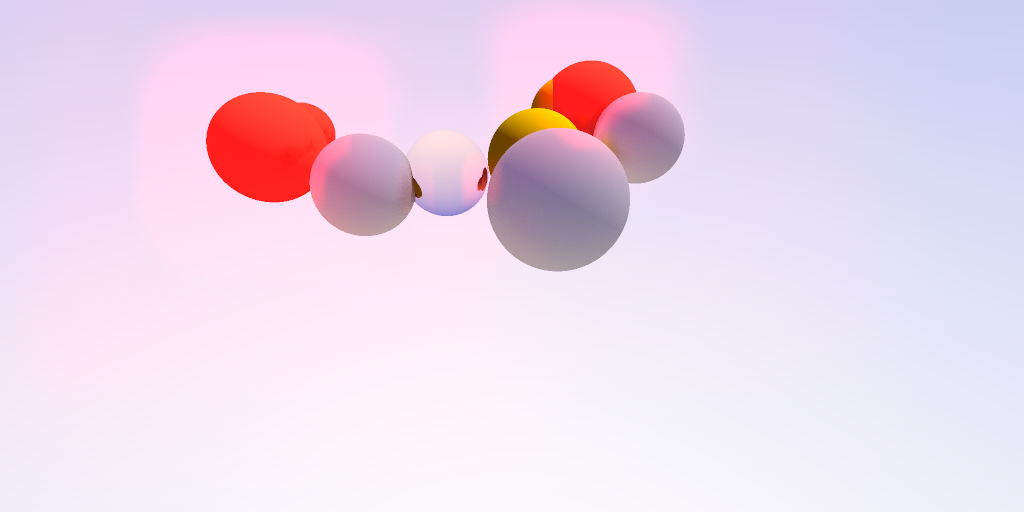
\includegraphics[width=0.8\textwidth]{RandomOutput.png}
  \caption{Scena randomica generata per il test}
  \label{fig:RandomOutput}
\end{figure}

Nella Figura \ref{fig:RandomOutput}, viene mostrato un esempio di scena 3D randomica generata dal nostro programma. Si noti che ogni esecuzione del programma produce una scena unica e dinamica.

\begin{figure}[htbp]
  \centering
  \begin{tikzpicture}
    \begin{axis}[
      width=0.8\textwidth,
      xlabel={Threads},
      ylabel={Speedup},
      xmin=0, xmax=20,
      ymin=0, ymax=10,
      xtick={2, 4, 6, 8, 10, 12, 14, 16, 18},
      ytick={0, 1, 2, 3, 4, 5, 6, 7, 8, 9, 10},
      legend pos=north east,
      grid style=dashed,
    ]
    \addplot[
      color=blue,
      mark=*,
      ]
      coordinates {
      (2, 1.874626)(4, 3.529136)(6, 4.706921)(8, 5.706580)(10, 6.097489)(12, 6.546816)(14, 6.880851)(16, 7.253451)(18, 7.449293)
      };
    \addlegendentry{SpeedUp}
    \label{SpeedUp}
    \end{axis}
    
    \begin{axis}[
      width=0.8\textwidth,
      axis y line*=right,
      axis x line=none,
      ylabel={Efficiency},
      xmin=0, xmax=20,
      ymin=0, ymax=100,
      xtick={2, 4, 6, 8, 10, 12, 14, 16, 18},
      ytick={0, 10, 20, 30, 40, 50, 60, 70, 80, 90, 100},
      legend pos=north east,
      grid style=dashed,
    ]
    \addlegendimage{/pgfplots/refstyle=SpeedUp}\addlegendentry{SpeedUp}
    \addplot[
      color=orange,
      mark=*,
      ]
      coordinates {
      (2, 93.73)(4, 88.23)(6, 78.45)(8, 71.33)(10, 60.98)(12, 54.56)(14, 49.15)(16, 45.33)(18, 41.39)
      };
    \addlegendentry{Efficiency}
    \end{axis}
  \end{tikzpicture}
  
  \caption{Grafico delle prestazioni del programma}
  \label{fig:performance_graph}
\end{figure}

\newpage
\begin{center}
\noindent
\resizebox{0.4\textwidth}{!}{%
\begin{tabular}{|c|c|c|}
\hline
\makecell{Threads} & \makecell{SpeedUp} & \makecell{Efficiency}\\
\hline
\hline
2 & 1.874626 & 93.73\\
4 & 3.529136 & 88.23\\
6 & 4.706921 & 78.45\\
8 & 5.706580 & 71.33\\
10 & 6.097489 & 60.98\\
12 & 6.546816 & 54.56\\
14 & 6.880851 & 49.15\\
16 & 7.253451 & 45.33\\
18 & 7.449293 & 41.39\\
\hline
\end{tabular}
}
\end{center}

Nel grafico riportato sopra possiamo osservare come le prestazioni variano al variare del numero dei threads.

\subsection{GPU}
\subsubsection{Benchmark al variare di Size e Samples}
Abbiamo valutato le prestazioni del sistema variando la dimensione dell'immagine e il numero di samples per pixel. Il Max Depth è stato impostato a 20 e la block size a 16x16px. Di seguito sono riportati i risultati:

\begin{center}
\begin{figure}[h]
    \centering
    \begin{adjustbox}{width=0.85\paperwidth,center}
    \includegraphics[width=0.85\paperwidth]{chart benchmark gpu renderer.png}
    \end{adjustbox}
\end{figure}
\end{center}
La tabella seguente mostra i tempi di rendering (in millisecondi) per diverse combinazioni di Size e Samples. I risultati sono suddivisi nelle fasi di Rendering e Applicazione dell'effetto di Glow:

\begin{center}
\noindent
\resizebox{\textwidth}{!}{%
\begin{tabular}{|l|c|c|c|c|c|c|c|c|c|}
\hline
 \makecell{Size\\Samples} & \makecell{512x256\\5} & \makecell{512x256\\10} & \makecell{512x256\\15} & \makecell{1024x512\\5} & \makecell{1024x512\\10} & \makecell{1024x512\\15} & \makecell{2048x1024\\5} & \makecell{2048x1024\\10} & \makecell{2048x1024\\15} \\
\hline
\hline
\coloredbox{6D2D6C}Rendering (ms) & 467 & 938 & 1315 & 765 & 1585 & 2228 & 1717 & 3466 & 5079 \\
\hline
\coloredbox{54AA5B}Glow (ms) & 40 & 40 & 40 & 45 & 45 & 45 & 56 & 56 & 56 \\
\hline
\end{tabular}
}
\end{center}

\newpage

\subsubsection{Bemchmark pre e post ottimizzazione di memoria}
Abbiamo inoltre valutato l'impatto del tipo di memoria sulle prestazioni di rendering. Per questi test, abbiamo fissato la dimensione dell'immagine a 512x256px, il numero di samples per pixel a 10, il MaxDepth a 20 e la block size a 16x16px.

\begin{center}
\begin{figure}[h]
    \centering
    \begin{adjustbox}{width=0.85\paperwidth,center}
    \includegraphics[width=0.85\paperwidth]{chart benchmark gpu renderer memory.png}
    \end{adjustbox}
\end{figure}
\end{center}

La tabella seguente riassume i tempi di rendering (in millisecondi) al variare del tipo di memoria usato:

\begin{center}
\resizebox{0.35\textwidth}{!}{%
\begin{tabular}{|l|c|c|}
\hline
\makecell{Memory} & \makecell{Global} & \makecell{Shared} \\
\hline
\hline
\coloredbox{6D2D6C}Blur & 2.6 &  \\
\hline
\coloredbox{D37C44}Blur H &  & 0.0915 \\
\hline
\coloredbox{36682F}Blur V &  & 0.0902 \\
\hline
\end{tabular}
}
\end{center}

L'analisi dei tempi di esecuzione per l'effetto di blur evidenzia significative differenze tra l'utilizzo della memoria globale e della memoria shared in ambiente CUDA. La tabella presentata mostra che l'operazione di blur totale, eseguita in memoria globale, richiede un tempo di 2.6 millisecondi. Questo valore è confrontato con l'approccio che utilizza la memoria shared, dove le operazioni di blur sono state suddivise in orizzontale (Blur H) e verticale (Blur V).

Notabilmente, l'implementazione con memoria shared mostra un drastico miglioramento nei tempi di esecuzione: solo 91.5 $\mu$s per il blur orizzontale e 90.2 $\mu$s per il blur verticale. Questi risultati sottolineano l'efficienza della memoria shared per operazioni che richiedono un elevato livello di accesso concorrente ai dati, riducendo significativamente il tempo di calcolo grazie alla riduzione dei colli di bottiglia nella lettura e scrittura dei dati.

L'ottimizzazione dell'effetto di blur mediante l'uso della memoria shared dimostra quindi come approcci adeguati alla gestione della memoria possano avere un impatto sostanziale sulle prestazioni complessive di algoritmi di elaborazione immagini su GPU.


\section{UML Diagram}
\begin{figure}[htbp]
  \centering
  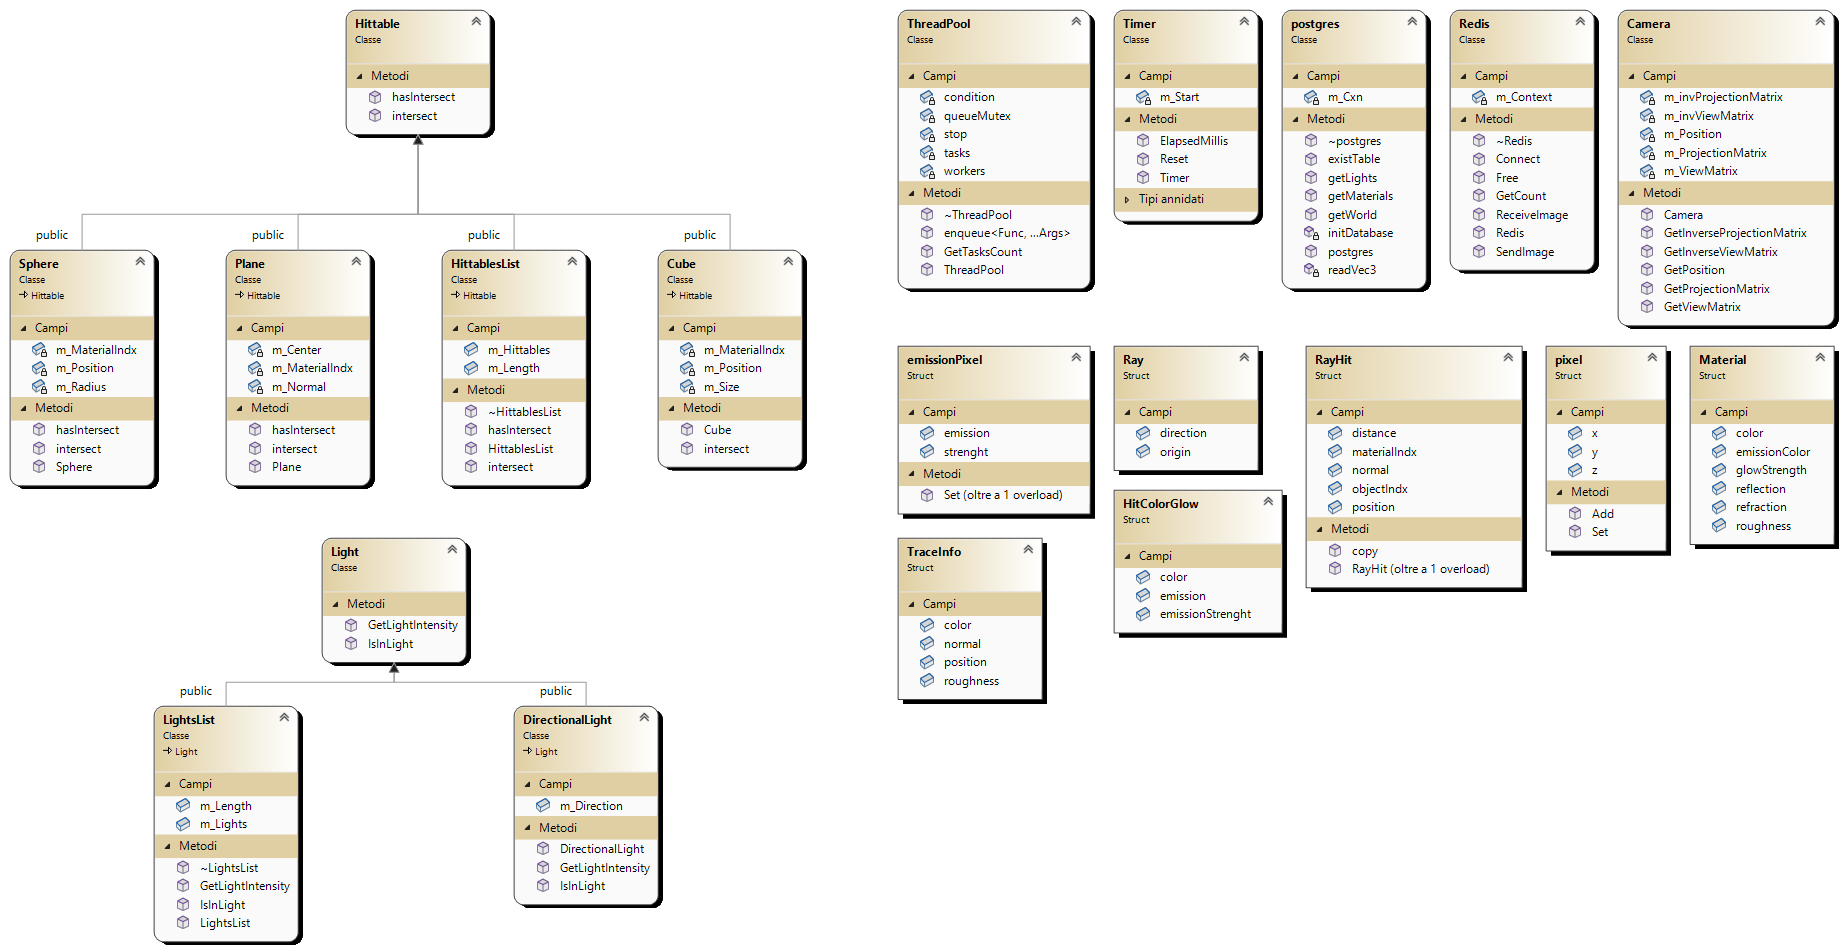
\includegraphics[width=1\textwidth]{ClassDiagram.png}
  \caption{Diagramma UML}
  \label{fig:uml_diagram}
\end{figure}

\newpage
\section{State Machine Diagram}
\begin{figure}[htbp]
  \centering
  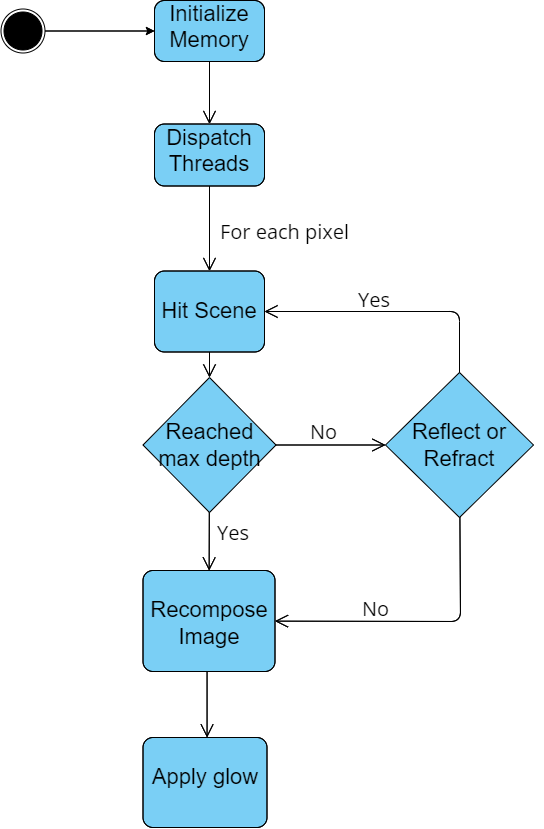
\includegraphics[width=0.7\textwidth]{StateMachineDiagram.png}
  \caption{State Machine Diagram}
  \label{fig:state_machine_diagram}
\end{figure}

\newpage
\section{Use Case Diagram}
\begin{figure}[htbp]
  \centering
  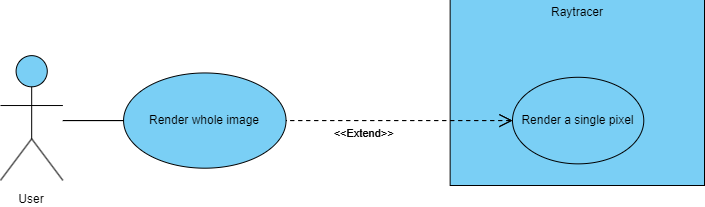
\includegraphics[width=0.8\textwidth]{UseCaseDiagram.png}
  \caption{Use Case Diagram}
  \label{fig:use_case_diagram}
\end{figure}

\section{Esempi di render}

\begin{figure}[htbp]
  \centering
  \includegraphics[width=0.75\textwidth]{Render1.png}
  \label{fig:render1}
\end{figure}

\begin{figure}[htbp]
  \centering
  \includegraphics[width=0.75\textwidth]{Render2.png}
  \label{fig:render1}
\end{figure}


\newpage
\section{Riferimenti}

\begin{thebibliography}{99}
\bibitem{riferimento1}
Peter Shirley,
\textit{Ray Tracing in One Weekend},
\url{https://raytracing.github.io/books/RayTracingInOneWeekend.html}

\bibitem{riferimento2}
Roger Allen,
\textit{Accelerated Ray Tracing in One Weekend in CUDA},
\url{https://developer.nvidia.com/blog/accelerated-ray-tracing-cuda/}

\bibitem{riferimento3}
\textit{OpenGL Camera},
\url{https://learnopengl.com/Getting-started/Camera}

\bibitem{riferimento4}
Robert Crovella,
\textit{Effective usage of Shared Memory},
\url{https://shorturl.at/qrMN3}

\end{thebibliography}
\end{document}
